\chapter{Eredmények értékelése}
A kidolgozott javaslatok esettanulmány alapján történő, illetve általános értékelése jelen fejezetben találhatóak.

\section{Kvadkopter esettanulmány}
A fent leírt módszerek tesztelése és továbbfejlesztése érdekében, szükség volt egy esettanulmányra, amelyen valóshoz hasonló körülmények közt is ki lehet próbálni az elméleti eredményeket.
Erre a célra egy olyan példa rendszerre van szükség, amely kellően bonyolult az előnyök kimutatására, az esetleges hiányosságok feltárására, de kezelhető méretű és lehetőleg széles körben érthető, hogy később demonstrációs eszközként szolgálhasson.

Ezek alapján a követelmények alapján egy kvadkopterre esett a választás. Pontosabban egy olyan négyrotoros drónra, amelynek az esettanulmányban a feladata, hogy szeles környezetben egy előre meghatározott pozícióban lebegjen.

Mivel az automatikus kódgenerálásra és a modellek konzisztenciájának ellenőrzésére még nincsenek eszközök, ezért ezeket a lépéseket manuálisan kellett elvégezni.
A következőkben először a rendszermodell, majd a szimulációs modell kerül bemutatásra, az elkészítésük során gyűjtött tapasztalatokkal együtt.

    \subsection{A rendszermodell}
    A rendszermodell esetében csak a főbb tervezési szempontok és a felépítés kerül bemutatásra, mert a dolgozat lényegének megértésében a konkrét forráskód elemzése nem segíti az olvasót. Ehelyett a struktúra bemutatása és a módszertan szempontjából lényeges részletek kiemelésére helyezem inkább a hangsúlyt ebben a részben.
    
    Az esettanulmány keretében a rendszer egy előre meghatározott pozíciót próbál tartani, így a kontextusmodellben csupán a szél jelenik meg külső befolyásoló elemként.
    A szelet a drón tömegközéppontjában ható erőként és forgatónyomatékként modelleztem, ezek mértéke az idő függvényében, a szimulációs modellben paraméterként adható meg, elősegítve a különböző terhelések vizsgálatát.

    A modellezett kvadkopter fizikailag igen egyszerű felépítést követ. Egy GPS és egy IMU modul segítségével méri a pozícióját és az orientációját. A példa egyszerűsége miatt ezek ideális szenzorként lettek modellezve.
    A módszertanban leírtak szerint ezt a modellt egy újabb iterációban lehetne tovább finomítani, de jelenleg tökéletesen megfelelő ez az absztrakció.
    
    A szenzorok adatait egy mikrokontroller olvassa, amely futtatja a szabályozó algoritmusokat, majd az azok eredményeképpen adódó motorvezérlő jeleket továbbküldi a négy motornak.
    
    A tervezés folyamán a motorokat kész komponensnek tekintettem amelyek a hozzájuk tartozó vezérlővel és rotorral egybeépítve készen kaphatóak. Ezek az egységek ipari drónok esetében valóban így kaphatóak katalógus szerint és saját adatlappal rendelkeznek, mert ezek a komponensek együtt határozzák meg a meghajtás különböző karakterisztikáit.
    Ezt azért fontos kiemelni, mert ez egy remek lehetőség kipróbálni a módszertanban javasolt könyvtárak használatát, illetve később a szimulációs modellben az FMU-k bemutatására is remek lehetőséget nyújt.
    
    A logikai modellben a szenzorok adatainak begyűjtése, a szabályozóalgoritmus és az az alapján történő beavatkozás jelenik meg magas szinten.
    
    Utóbbi kettő azért érdekes, mert így a magasszintű modellben nem köteleződtünk el egy konkrét implementáció mellett, mivel számos megvalósítás lehetséges egy forgószárnyas drón megvalósítására. Ennek az előnye többek között, hogy a pozíciótartásért felelős szabályozó csak az összesített tolóerőt és a különböző forgástengelyek mentén jelentkező elmozdulást állítja így ez gyakorlatilag teljesen független a rotorok számától és elhelyezkedésétől.
    Ez persze azt jelenti, hogy a szabályozó kimenetét nem lehet azonnal a motoroknak küldeni, hanem előbb elő kell állítani belőlük a konkrét beavatkozószervek utasításait.
    
    Ezzel a megoldással a szabályozónk újrahasználható elemmé vált, amelyet csak paraméterezni kell egy új hasonló rendszer esetében, ami egy valós projektnél előnyös gyakorlatnak számítana.
    
    Ezek alapján a beavatkozó blokk a későbbiekben tovább lett finomítva, hogy az általános parancsok alapján meghatározza az egyes motorok tolóerejét az adott konfigurációhoz. 
    Ezzel együtt finomításra került a két adatgyűjtési feladat a konkrét mérésre, valamint annak a szenzorból való kiolvasására és feldolgozására.
    
    Ennél a két esetnél jól megfigyelhető hogy a logikai és fizikai elemek átlapolódnak. Az adatgyűjtés két fizikai elemet is érintett, a beavatkozás pedig ötöt is, a transzformáció és a négy motor vezérlése által.
    
    Ezek az átlapolódások jól láthatóak voltak a magasszintű allokációk elkészítésénél, a következő fázisban a felhasználásikkal egyszerűen, egy lépésben elvégezhető volt a modellek finomítása az iteratív próbálkozás elkerülésével.


    \subsection{A szimulációs modell}
    A rendszer fejlődésével készült egy a rendszert egyben reprezentáló szimulációs modell, amely a logikai és fizikai vetületet együtt reprezentálja az allokációnak megfelelően.
    
    Ez alapján készült el később a Modelica modell is az eszköz beépített blokk-könyvtárával, amellyel grafikusan is megadhatóak a nyelv elemei.
    
    A szimulációk alkalmazására a motorok paramétereinek kiválasztását használtam fel példaként. A követelmény az volt, hogy a drón $0.02N$ erőt és $0.02Nm$ forgatónyomatékot kifejtő szél mellett is maximum $0.01m$ kitéréssel tudja tartani a megadott pozíciót.
    A szimulációk szerepe az volt, hogy megadott motorok közül szimulációk segítségével választottam ki azt, amelyik képes volt tartani ezt a követelményt.

    Mivel a dolgozatban egyaránt foglalkoztam az FMU-kkal kompatibilis és a megkötések nélküli szimulációs modellekkel, ezért mindkét módszerrel készült egy-egy szimulációs modell.
    A megértést megkönnyítendő, a két modellben a különböző blokkokat eltérő színnel és betűjellel jelöltem az alábbiak szerint:

    \begin{description}
        \item[Mikrokontroller] C(ontroller) narancssárga színnel
        \item[Motor] M(otor) világoszöld színnel
        \item[Váz] F(rame) világoskék színnel
        \item[Szenzorok] S(ensors) lila színnel
    \end{description}

    A szerkesztő által használt jelölések a kapcsolatokhoz:

    \begin{description}
        \item[Számadatok] Kék vonalak és háromszög alakú csatlakozók, valós számok átadására.
        \item[Mechanika] Szürke vonalak és szögletes csatlakozók, az erők és forgatónyomatékok mindkét irányban terjednek rajtuk.
    \end{description}

        \subsubsection{Megkötések nélküli verzió}
        Ezt a modellt egyszerűen lehetett származtatni a rendszermodellből. Mivel a Modelica is lehetővé teszi a hierarchikus tervezést, ezért ezt a módszert alkalmaztam az átláthatóság érdekében.
        A hierarchia tetején a fizikai komponensek helyezkednek el, ezek belsejében vannak a logikai komponensek, amelyek a belső működést definiálják, illetve az adott alkatrész fizikai modellje is.
        Ezzel egy könnyen követhető modellstruktúrát kaptam, amely könnyen áttekinthető. A rendszernek ez a virtuális reprezentációja szerkezetileg alapvetően megegyezik a valóssal.
        Ez megfelel annak az elképzelésnek, hogy a szimulációs modell egy virtuális mása a valódi rendszernek.

        A modell a fentiekben leírt jelöléseknek megfelelően a \ref{fig:stdSzim} ábrán látható.
        Jól megfigyelhető, hogy a motorok, szenzorok és a drón váza mechanikai kapcsolatban állnak egymással.
        Ugyanakkor a mikrokontroller a szenzorokkal és a motorokkal számadatokkal kommunikál.
        Természetesen a valóságban a mikrokontroller is a géphez lenne rögzítve, de ebben az egyszerűsített modellben a tömegét elhanyagoltam, az ábra áttekinthetősége érdekében.

        \begin{figure}[!ht]
            \centering
            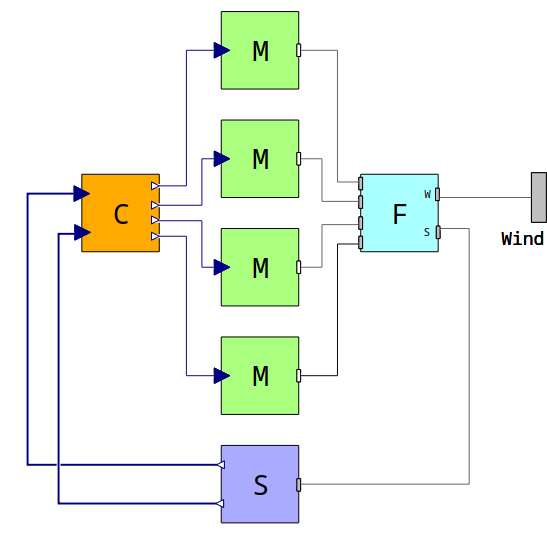
\includegraphics[width=100mm, keepaspectratio]{figures/stdSzim.png}
            \caption{A megkötések nélkül elkészített szimulációs modell.} 
            \label{fig:stdSzim}
        \end{figure}

        \subsubsection{FMI kompatibilis verzió}
        Ennek a modellnek a különlegessége, hogy míg az előzőben használható volt olyan kapcsolat, amely azt írta le, hogy a motorok fizikai kapcsolatban állnak a drón vázával, addig ebben a verzióban a komponensek határán csak logikai értékek valamint egész és racionális számok léphettek át.
        Ez persze feloldható volt a \ref{sec:fmiKompat} részben leírt módszerrel, azonban ennek következtében a motorok és a váz között nem egy mechanikai kapcsolat volt, amin a megfelelő értékek minkét irányba terjedhettek, hanem az adott motor keltette tolóerő és forgatónyomaték, amely a váz modelljén belül került átalakításra fizikai értékké. Ennek következtében az, hogy minden motor mozgása kihat a teljes rendszerre, csak úgy volt modellezhető, hogy a mozgásmodell teljesen a vázban került megvalósításra.

        Ennek kellemetlen következménye, hogy a motorok tömegét modellező blokkokat a vázban kellett elhelyezni, pedig ez egy külön alkatrész ami le is cserélhető egy másikra.
        Persze megoldható, hogy paraméterként adhassuk meg és az SSP (Lásd: \ref{sec:ssp} rész) szabvánnyal elméletben megoldható, hogy egy adott katalógusból választott motortípus kiválasztásával az egész modell átparaméterezhető legyen, de ez olyan komplex probléma ami nehezen automatizálható, sok hibalehetőséget tartalmaz és nehezen újrahasználható illetve karbantartható modellekhez vezet.

        Az, hogy egy komponens modellje részben egy másikba kerül áthelyezésre, és nem a valós kapcsolatokat látjuk, hanem számértékek terjedését, nagyban megnehezíti annak áttekintését és felhasználását, de cserébe megoldható a modellek átadása anélkül, hogy a gyártó felfedné az implementáció részleteit, ami több ipari résztvevő között gyakran megjelenő igény a közös munka során.
        Mindemellett amíg a szabványt nem bővítik a szükséges akauzális kapcsolatok leírásához szükséges megoldásokkal, addig ez a technika csak nagyon indokolt esetben javasolt.

        Az FMI kompatibilis modell a fentiekben leírt jelöléseknek megfelelően a \ref{fig:fmiSzim} ábrán látható.
        Megfigyelhető, hogy az előző modellhez képest itt kizárólag számadatok formájában áramlik adat a komponensek között.
        A szenzorok esetében a mérést végző blokkok a vázba kerültek és a \emph{Sensors} blokk csak a szenzorra jellemző zajt és egyéb paramétereket modellezi.
        A \emph{Motor} blokkok pedig kizárólag az általuk létrehozott mechanikai hatások mértékét továbbítja a váznak amely a teljes dinamikai modellt implementálja, beleértve a határain kívül eső blokkok szerepét is.

        \begin{figure}[!ht]
            \centering
            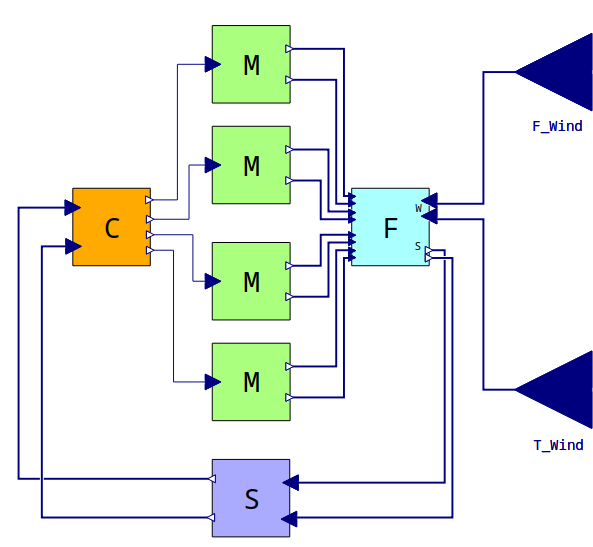
\includegraphics[width=100mm, keepaspectratio]{figures/fmiSzim.png}
            \caption{Az FMI szabvány megkötései szerint elkészített szimulációs modell.} 
            \label{fig:fmiSzim}
        \end{figure}

        \subsubsection{Szimulációs eredmények}
            \paragraph{Prototipizálás és validáció}
            A fejlesztés során a szimulációk segítségével választottam ki azokat a motorparamétereket, amelyekkel már megfelelő pontossággal garantálható volt a pozíciótartás.
            Az esettanulmány keretében ez azt jelentette, hogy minden méréshez manuálisan kellett átparaméterezni a szimulációs modellt és a gyűjtött adatokat manuálisan kiértékelni. Ez egy ilyen egyszerű példa keretében is időigényes feladat volt manuálisan, azonban nem igényelte  az összes motorvariáns és a többi alkatrész beszerzését és prototípusok gyártását, ahogy egy szélcsatorna használatát sem.

            A modellek automatikus generálásával ez a folyamat mindössze a mérési összeállítás és a követelmények modellezését tenné szükségessé, a mérések elvégzése és kiértékelése már teljesen automatizáltan történhetne, lehetővé téve több alternatíva gyors vizsgálatát.
            Fontos megemlíteni, hogy a követelmények és a mérési összeállítások modelljének egyébként is meg kell jelenni a rendszermodellben, mivel ez elengedhetetlen a nyomonkövethetőség biztosításához és a mérések megismételhetőségéhez.

            \paragraph{Végleges validáció}
            A fejlesztést befejezve, az utolsó lépés a végleges szimulációs modellek segítségével a modell validálása volt. A szimulációkat futtatva a rendszer mindkét modell esetében felemelkedett, megközelítette az előre kijelölt pozíciót és azt a széllökések mellett is tartotta elfogadható mértékű kitérések mellett.
            
            A szimulációs eredményeket szemléltető animációról készült képek a \ref{fig:SimRes} ábrán láthatóak.
            Az ábrán a fekete elemek a referencia koordináta-rendszert, a kékek magát a kvadkoptert, míg a zöldek az erőket és forgatónyomatékokat szemléltetik.
            A szélső, motorokat jelképező gömbökre hatóerők és forgatónyomatékok a motorok által keltettek, amelyekkel beavatkozunk a rendszerbe. Az origóból induló lefelé mutató erő a gravitációt reprezentálja.
            A kvadkopter testén ható erő és forgatónyomaték, amely az ábrán látható módon a többi nyíltól függetlenül mozog, a rendszerre ható szélzavarást reprezentálja.

            A szimuláció paraméterei úgy lettek meghatározva, hogy a rendszer az origóból felszállva az $y$ tengelyt jelképező nyíl hegyénél lebegjen.
            
            Az ábrán látható, hogy a rendszer a szimuláció második felében -öt másodperc után- már elérte a kitűzött célt, a továbbiakban ezt próbálja tartani a szélzavarás ellenére, ez okozza a harmadik és negyedik képen látható kitéréseket.
            Ezeknek az eredményeknek az alapján, a tervezési folyamat és az esettanulmány is sikeresnek tekinthető.

            \begin{figure}[!ht]
                \centering
                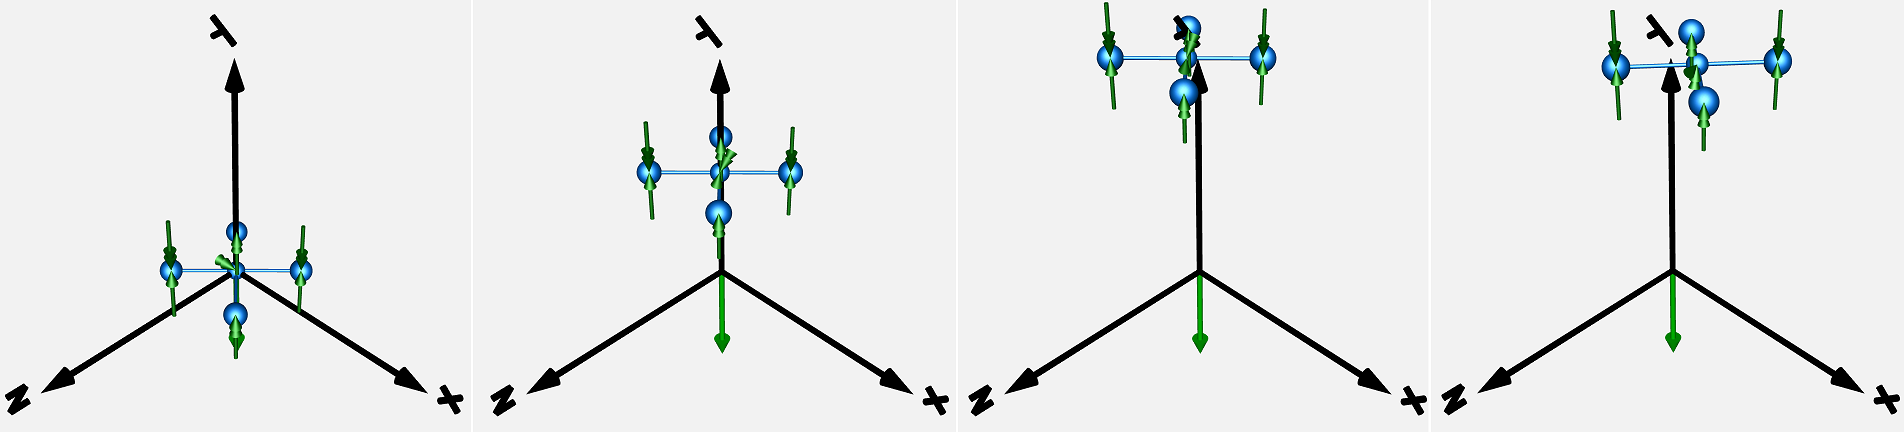
\includegraphics[width=150mm, keepaspectratio]{figures/SimRes.png}
                \caption{A szimulációk eredménye pillanatképeken.}
                \label{fig:SimRes}
            \end{figure}

    \section{Értékelés a motivációk szempontjából}
    Először érdemes megvizsgálni, hogy a dolgozat motivációjául szolgáló szempontok szerint mennyire eredményes az eddigi munka.

        \subsection{Rendszertervezési szempontok}
        A modellalapú technikák általános előnyei közzé tartozik a nyomonkövethetőség, a modellek konzisztenciája és a nézetek és dokumentumok automatikus generálhatósága.
        Mivel a dolgozatban javasolt módszertan is ilyen, modellalapú megközelítést alkalmaz, ezért ezeket nyelvi szinten teljesíti, illetve kompatibilis az eszközökkel amik képeset teljesíteni a konzisztencia esetében.
        A következő szempontok azok, amelyekre csupán lehetőséget biztosít a technológia, de ezek megvalósítása már a módszertannak köszönhető.

            \paragraph{Validáció és Verifikáció (V\&V) minden fejlesztési fázisban} \label{ertekelesVV}
            A módszertan bemutatása során látható volt, hogy a fejlesztés folyamán több alkalommal is szerepelnek validációs lépések, melyeknek célja a hibák mielőbbi kiszűrése.
            Ez komoly előrelépés a hagyományos módszerekhez és több modellalapú módszertanhoz képest, amelyek nem, vagy csak a fejlesztés végén tartalmaznak ilyen elemeket. (Lásd: \ref{sec:KorabbiModszerek} rész)
            Jelen dolgozat a szimulációs technológiákkal kapcsolatos validációra koncentrált, de természetesen ezekkel együtt végrehajthatóak más V\&V lépések is ugyanazokon a pontokon.

            \paragraph{Modellek újrahasználhatósága}
            A javasolt módszerek kitértek olyan könyvtárak használatára amelyek újrahasználhatóvá teszik az általános modellrészleteket.
            Ez a szempont jellemzően nem jelent meg az eddigi módszertanokban, bár természetesen nem is zárták ki ezek használatát. (Lásd: \ref{sec:KorabbiModszerek} rész)
            A javasolt megközelítés esetén kiemelendő, hogy a szimulációs technológiákkal integrált könyvtárakat javasol. Ezeknek a könyvtárba rendezése összhangban áll az általános szimulációs törekvésekkel és még inkább elősegíti a két terület integrálását.

        \subsection{Szimulációs szempontok}
        Mivel a módszertan lehetőséget nyújt a szimulációs technológiák alkalmazására, így magában foglalja azok előnyeit is.
        Meg kell említeni azonban, hogy bár a dolgozat kitért a HiL illetve SiL szimulációkkal való kompatibilitásra és elvi szinten támogatja azokat, ennek pontos megvalósításával nem volt lehetőség foglalkozni az eddigi munka során.

        \subsection{A két technológia integrálása szerint}
        Látható, hogy a kidolgozott módszerek számos előnnyel rendelkezik a két érintett terület kapcsán, azonban célja a kettő ötvözése, az alábbiakban egyesével értékelem az ennek kapcsán felmerült előrelépéseket és hiányosságokat.

            \paragraph{Szimulációs modellek automatikus generálása}
            Mivel a két terület integrálásához szükséges a rendszermodellben egy külön reprezentációt készíteni a szimulációs modellekhez, ezért felmerül az igény, hogy ezek alapján automatikusan állítsuk elő őket.
            
            A módszertan kidolgozása során részletesen vizsgáltam ezt a lehetőséget és kidolgozásra kerültek ennek alapvető sémái. Ezek az eredmények azért nem szerepeltek o dolgozatban, mert először későbbi fejlesztésre lettek félretéve, később pedig rábukkantam a \ref{sec:SysPhS} részben bemutatott SysPhS
            szabványra, amely az elérhető leírások alapján illeszkedik a kidolgozott alapelvekhez, így a saját megoldás helyett a két technológia ötvözése lett a cél ezen a területen.
            
            Az esettanulmány alatt, amikor a szimulációs modellreprezentációkat és a szimulációs modelleket is kézzel kellett elkészítenem, az eddigiek mellett felmerült, hogy magukat a modellreprezentációkat is lehetne részben automatikusan generálni, ezzel még jobban kiterjesztve ezeket az előnyöket.

            \paragraph{Munkafolyamatok konzisztenciájának garantálása}
            Az integrált technikák esetében ez a cél különböző modelltípusok konzisztenciáját jelenti. A módszertan javaslatot tett olyan modellstruktúrákra, amelyek megkönnyítik ennek ellenőrzését, illetve lehetőséget biztosít a kódgenerálásra, amely biztosítja ennek a konzisztenciának a felhasználóbarát megvalósítását is.
            
            Ami a szimulációk eredményeit illeti, ezeknek a garantált konzisztenciájához szükséges, hogy a szimuláció eredménye automatikusan visszakerüljön a rendszermodellbe.
            A leképezés ezen irányára nem tért ki a módszertan, bár az esettanulmány tapasztalatai alapján ez módszertantól független eszközökkel biztosítható, ha a tervezési folyamatban van hely ilyen vizsgálatoknak.
            A \ref{sec:flow} rész végén találhatóak javaslatok ilyen lépések elhelyezésére, így egy ilyen eszköz elméletileg gond nélkül használható a javasolt módszerekkel.

            \paragraph{Integrált V\&V}
            A két előző pont teljesülése esetén megvalósuló integrált V\&V folyamatok a fentiekben leírtak alapján elő lettek készítve, azonban tényleges megvalósításuk még várat magára, főleg mivel ehhez már szükség van az említett kétirányú kapcsolatra.
            
            \paragraph{Rendszer-identifikáció támogatása paraméter-visszavetítéssel}
            Ez a technológia ugyanarra a kétirányú kapcsolatra támaszkodik mint ami az előző két pontban is szerepelt, így ennek megvalósítása szintén külső eszközök fejlesztését igényli, de a tapasztalatok alapján, ha elkészülnek ilyen keretrendszerek, akkor azok használhatóak lesznek a leírt módszerekkel.

    \section{Értékelés a felhasználási tapasztalatok szerint}
    Az esettanulmány során készített modellek fejlesztésénél a leírt módszerek hatékonynak és kényelmesnek bizonyultak.
    
    A szimulációs modelltranszformáció alapvetően repetitív és monoton feladatnak bizonyultak, ahogy azt a \ref{sec:ReMoOsszehasonlitas} részben előrevetítettem, azonban ennek az elvégzése hosszútávon automatizálandó feladatként szerepelt a kezdetektől fogva.
    A tapasztalatok alapján ez a feladat valóban sematikus és jól automatizálható.
    
    A finomítások során szükséges adatok könnyen kinyerhetőek a javasolt allokáció-centrikus modellekből, nemcsak a tervezők, de az automatizált eszközök számára is. Mindkét eset megkönnyíthető lenne viszont nyelvi kiterjesztések használatával, amely érdekes továbbhaladási irányt jelent.